\chapter{Radionuclides}

In nuclear medicine, a tracer molecule is administered to the patient, usually
by intravenous injection. A tracer is a particular molecule, carrying an
unstable isotope, a radionuclide. The molecule is recognized by the body, and
will get involved in some metabolic process. The unstable isotopes produce
gamma rays, which allow us to measure the concentration of the tracer molecule
in the body as a function of position and time. A tracer is always administered
in very low amounts, such that the natural process being studied is not
affected by the tracer.

Consequently, nuclear medicine is all about {\em measuring function or
metabolism}, in contrast to many other modalities including CT, MRI and
echography, which mainly perform anatomical measurements. This boundary is not
strict, though: CT, MRI and ultrasound imaging allow functional measurements,
while nuclear medicine instruments also provide some anatomical information.
However, nuclear medicine techniques provide concentration measurements with a
sensitivity that is orders of magnitude higher than that of any other
modality.

\section{Radioactive decay modes}
%%%%%%%%%%%%%%%%%%%%%%%%%%%%%%%%%
The radionuclides emit electromagnetic rays during radioactive decay. These
rays are called ``gamma rays'' or ``X-rays''.  Usually, electromagnetic rays
originating from nuclei are called gamma rays, while those from atoms are
called x-rays. However, when they have the same frequency they are
indistinguishable. The energy of a photon equals
\begin{align}
   E &= h\nu = \frac{hc}{\lambda}\\
   h &= 6.626 \cdot 10^{-34} \mbox{ J} 
   \;\;=\;\; 4.136\cdot 10^{-15} \mbox{ eV}\\
   c &= 30 \mbox{ cm/ns}
\end{align}
where $h$ is the Planck constant, $c$ is the speed of light, $\nu$ the
frequency and $\lambda$ the wavelength of the photon. The ratio
between electronvolt and joule is numerically equal to the unit of
charge in coulomb: $e = 1.602\cdot 10^{-19}$ C. Visible light has a
wavelength of about 400 to 700 nm, and therefore an energy of about
4.1 to 1.8 eV. The gamma rays used in nuclear medicine have energies
of 100 to 600 keV, corresponding to wavelengths of a few pm.

There are many ways in which unstable isotopes can decay. Depending on
the decay mode, one or more gamma rays will be emitted in every
event. Some isotopes may use different decay modes. The probability of
each mode is called the {\em branching ratio}. As an example, $^{18}$F
has a branching ratio of 0.97 for positron decay, and a branching
ratio of 0.03 for electron capture.
\begin{enumerate}

\item $\beta^-$ emission.
%
\begin{itemize}
\item
In this process, a neutron is transformed into a proton and an
electron (called a $\beta^-$ particle).  Also a neutrino (an electron
anti-neutrino $\bar\nu_e$) is produced and (since the decay result is
more stable) some energy is released:
\begin{equation}
 n \rightarrow p^+ + e^- + \bar\nu_e \ .
\end{equation}
Since the number of protons is increased, this transmutation process
corresponds to a rightward step in Mendeleev's table.

\item
The resulting daughter product of the above transmutation can also be in an
excited state, in which case it rapidly decays to a more stable nuclear
arrangement, releasing the excess energy as one or more $\gamma$ photons.  The
nucleons are unchanged, so there is no additional transmutation in decay from
excited to ground state.

\item
The daughter nucleus of the decay process may also be in a metastable or
isomeric state. In contrast to an excited state, the life time of a metastable
state is ``much longer''
\footnote{The boundary between excited and metastable is usually said
  to be about $10^{-9}$ s, which is rather short in practice. But the
  half life of some isomers is in the order of days or years.}.  
%
When it finally decays, it does so by emitting a photon. In many
metastable isotopes, this photon may be immediately absorbed by an
electron of the very same atom, as a result of which that electron is
ejected.  This is called a (internal) conversion electron. The kinetic
energy of the ejected electron is equal to the difference between the
energy of the photon and the electron binding energy. 

The most important single photon isotope \textsuperscript{99m}Tc\ is an example of this
mode. \textsuperscript{99m}Tc\ is a metastable daughter product of $^{99}$Mo (half life 66
hours). \textsuperscript{99m}Tc\ decays to $^{99}$Tc (half life 6 hours) by emitting a
photon of 140 keV. $^{99}$Mo is produced in a fission reactor
\footnote{There are only 5 places worldwide where $^{99}$Mo is
  produced (one in Mol, Belgium, one in Petten, the Netherlands), and
  4 where it can be processed to produce \textsuperscript{99m}Tc\ generators (one in
  Petten, one in Fleurus, Belgium).}.
\end{itemize}

\item Electron capture (EC).
\begin{itemize}
\item An orbital electron is captured, and combined with a proton to produce a
neutron and an electron neutrino:
\begin{equation}
  p^+ + e^- \rightarrow n + \nu_e
\end{equation}
As a result of this, there is an orbital electron vacancy.  An electron from a
higher orbit will fill this vacancy, emitting the excess energy as a photon.
Note that EC causes transmutation towards the leftmost neighbor in
Mendeleev's table.

\item If the daughter product is in an excited state, it will further decay
towards a state with lower energy by emitting additional energy as $\gamma$
photons (or conversion electrons).

\item
Similarly, the daughter product may be metastable, decaying via isomeric
transition after a longer time.
\end{itemize}

Examples of radionuclides decaying with EC are $^{57}$Co, $^{111}$In,
$^{123}$I and $^{201}$Tl. Figure \ref{fig:In111} shows the decay
scheme for $^{111}$In and (a small part of) the decay
table. Conversion electrons are denoted with ``ce-$X$, $y$'', where
$X$ is the electron shell and $y$ is the gamma ray. The table also
gives the kinetic energy of the conversion electron, which must of
course be less than the energy of the photon that produced it. The
ejection of the conversion electron creates a vacancy in the involved
electron shell, which is filled by an electron from a higher
shell. The excess energy is released as an X-ray or as an Auger
electron. In the decay table, X-rays are denoted with ``$Xa$ X-ray'',
where $X$ is the electron shell that had a vacancy, and $a$ says (in
code) from which shell the new electron comes. The energy of this
X-ray exactly equals the difference between the energies of the two
electron shells.  Instead of emitting an X-ray, the excess energy can
be used to emit another electron from the atom. This is called the
Auger-effect, and the emitted electron is called an Auger-electron. In
the table an Auger electron is denoted as ``Auger-$XYZ$'', if a
vacancy in shell $X$ is filled by an electron from shell $Y$, using
the excess energy to emit an electron from shell $Z$. The table gives
the kinetic energy of the emitted Auger-electron. The table also gives
the frequency, i.e. the probability that each particular emission
occurs when the isotope decays.
%
%% \begin{figure}[htb]
%% \centering
%% \figbox{0.9\textwidth}{fig_In111.eps}
%% \caption{\label{fig:In111} \emph{Decay scheme of $^{111}$In, by
%%     electron capture. The scheme is dominated by the emission of two
%%     gamma rays (171 and 245 keV). These gamma rays can be involved in
%%     production of conversion electrons. A more complete table is given
%%     in \cite{Cherry}.}}
%% \end{figure}

\begin{figure}[htb]
\centering
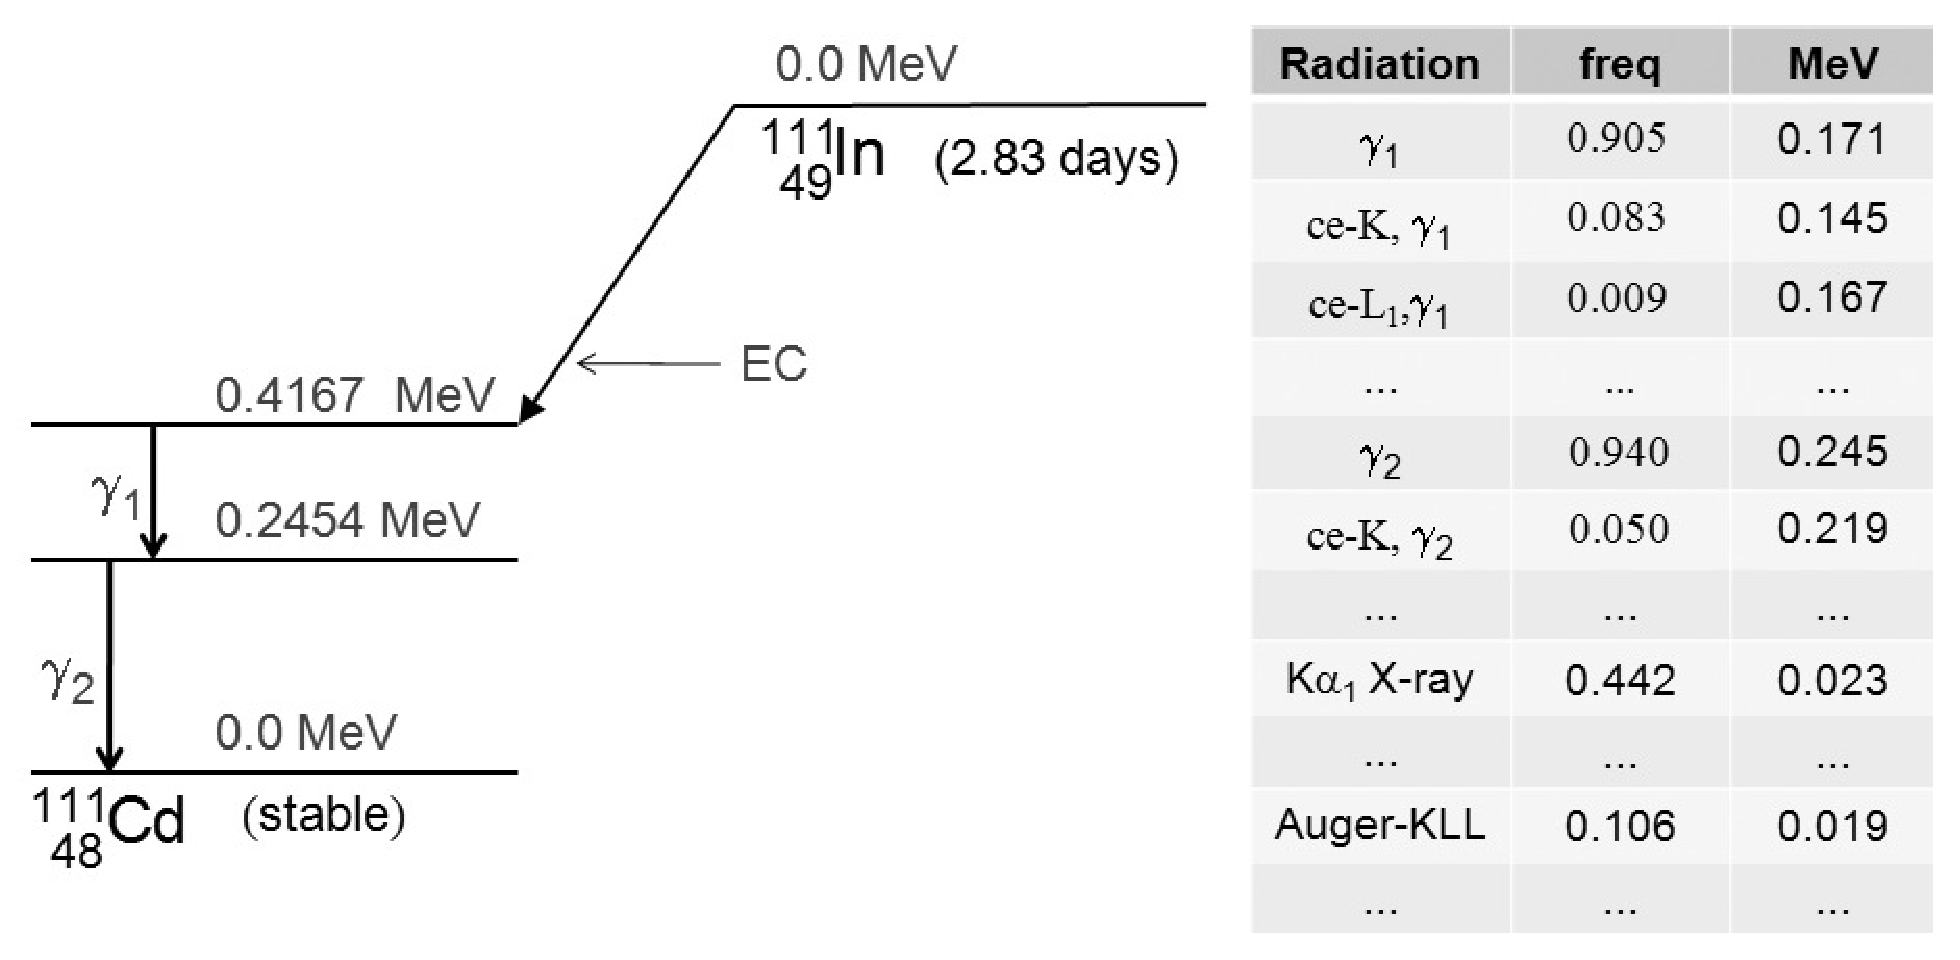
\includegraphics[width = 0.8\textwidth]{figs/fig_In111.pdf}
\caption{\label{fig:In111} \emph{Decay scheme of $^{111}$In, by
    electron capture. The scheme is dominated by the emission of two
    gamma rays (171 and 245 keV). These gamma rays can be involved in
    production of conversion electrons. A more complete table is given
    in \cite{Cherry}.}}
\end{figure}

\item Positron emission ($\beta^+$ decay).\\
\begin{itemize}
\item A proton is transformed into a neutron and a positron (or
anti-electron):
\begin{equation}
  p^+ \rightarrow n + e^+ + \nu_e \ .
\end{equation}
After a very short time the positron will hit an electron and annihilate
(fig. \ref{fig:jnpos}).  The mass of the two particles is converted into
energy, which is emitted as two photons. These photons are emitted in opposite
directions. Each photon has an energy of 511 keV (the rest mass of an electron
or positron).


\begin{figure}[tb]
\centering
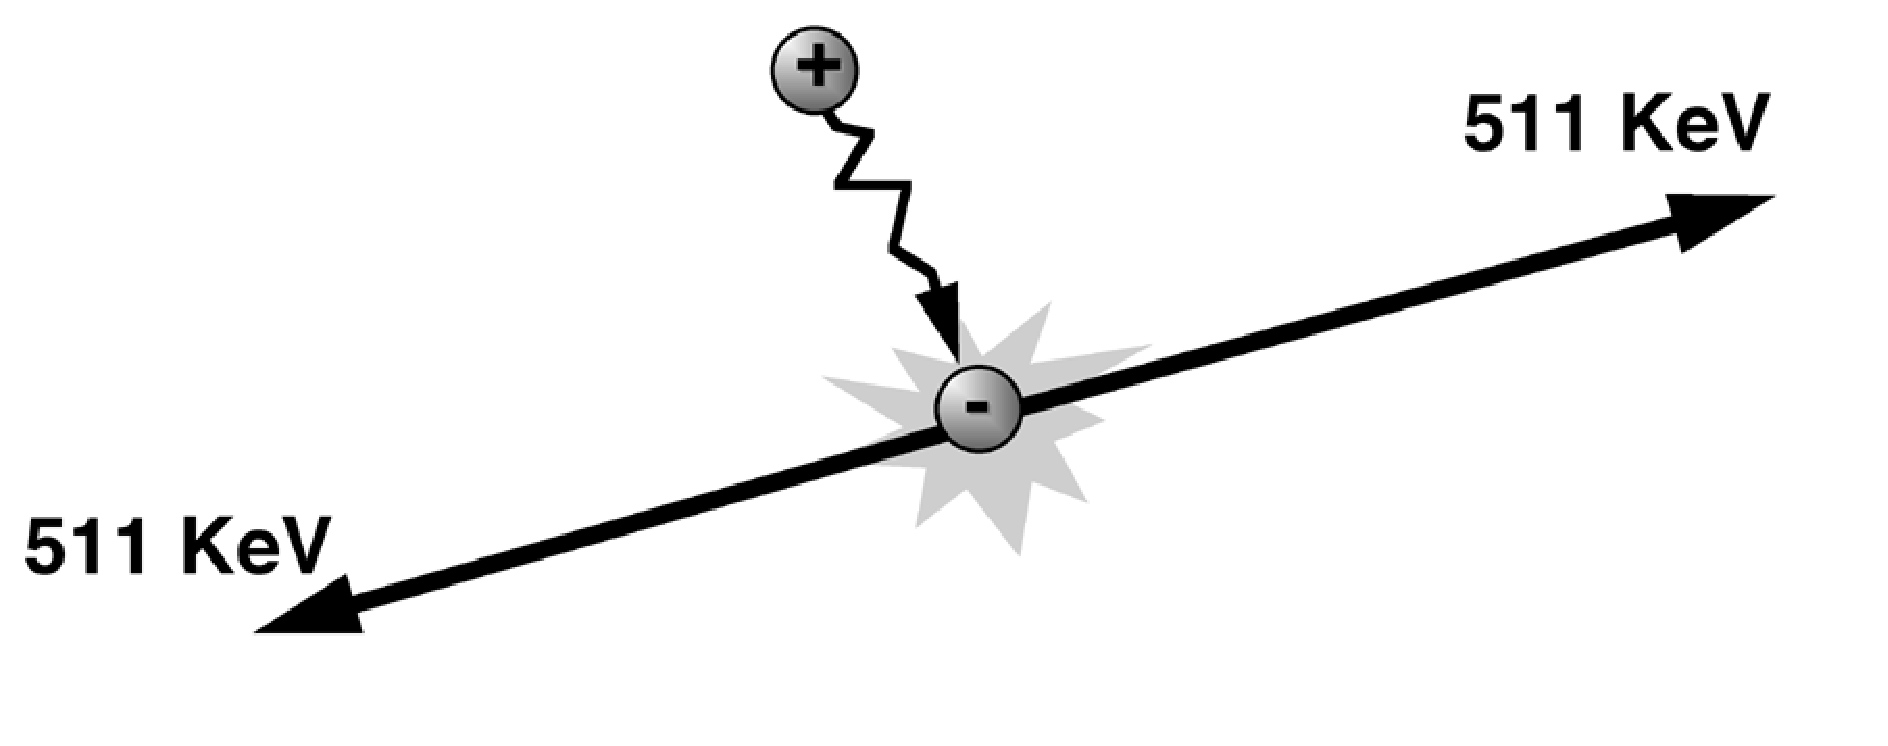
\includegraphics[width = 0.5\textwidth]{figs/fig_jnpos.pdf}
\caption{\emph{Positron-electron annihilation.}}
\label{fig:jnpos} 
\end{figure}


\item Again, the daughter nucleus may also be in an excited or a metastable
state.

\end{itemize}
\end{enumerate}
As a rule of thumb, light atoms tend to emit positrons, heavy ones
tend to prefer other modes, but there are exceptions. The most
important isotopes used for positron emission imaging are $^{11}$C,
$^{13}$N, $^{15}$O and $^{18}$F. Since these atoms are very frequent
in biological molecules, it is possible to make a radioactive tracer
which is chemically identical to the target molecule, by substitution
of a stable atom by the corresponding radioactive isotope. These
isotopes are relatively short lived: $^{11}$C: 20 min, $^{13}$N: 10
min, $^{15}$O: 2 min and $^{18}$F: 2 hours. As a result, except for
$^{18}$F, they must be produced close to the PET-system immediately
before injection. To produce the isotope, a small cyclotron is
required. The isotope must be rapidly incorporated into the tracer
molecule in a dedicated radiopharmacy laboratory. In contrast,
$^{18}$F can be transported from the production site to the
hospital. That makes it the most popular isotope in PET.

In nuclear medicine, we use radioactive isotopes that emit photons with an
energy between 80 and 300 keV for single photon emission, and 511 keV for
positron emission. The energy of the emitted photons is fixed: each isotope
emits photons with one or a few very sharp energy peaks. If more than one peak
is present, each one has its own probability which is a constant for that
isotope. So if we administer a tracer to a patient, we know exactly what
photons we will have to measure.


\section{Statistics} \label{sec:statistics}
%%%%%%%%%%%%%%%%%%%%%%%%%%%%%%%%%
The exact moment at which an atom will decay cannot be predicted. All that is
known is the probability that it will decay in the next time interval $dt$.
This probability is $\alpha dt$, where $\alpha$ is a constant for each
isotope.  So if we have $N$ radioactive atoms at time $t_0$, we expect to
see a decrease $dN$ in the next interval $dt$ of
\begin{equation}
  dN = - N \alpha dt. \label{eq:dN}
\end{equation}
Integration over time yields
\begin{equation}
  N(t) = N(t_0) e^{- \alpha (t - t_0)}. \label{jn:decay}
\end{equation}
This is what we {\em expect}. If we actually measure it, we may obtain a
different value, since the process is statistical. As shown below, the
estimate will be better for larger $dN/dt$.

The amount of radioactivity is not expressed as the number of
radioactive atoms present, but as the number of radioactive atoms
decaying per unit of time. From (\ref{eq:dN}) we find that
\begin{equation}
  \mbox{radioactivity} = -\frac{dN}{dt} = \alpha N =
  \frac{N}{t_{\frac{1}{2}}} \ln 2.
\end{equation}
Therefore, for the same amount of radioactivity, more radioactive
atoms are needed if the half life is longer.  This quantity used to be
expressed in Curie (Ci), but the preferred unit is now Becquerel (Bq)
\footnote{Marie and Pierre Curie and Antoine Becquerel received the
Nobel prize in 1903, for their discovery of radioactivity in 1896}.
One Bq means 1 event per s. For the coming years, it is useful to know
that
\begin{equation}
 1 \ \mbox{mCi} = 37 \ \mbox{MBq} = 37 \times 10^{6} / \mbox{s}.
\end{equation}
The amounts of radioactivity used in nuclear medicine imaging are
typically in the order of $10^2$ Mbq.

The half life of a tracer is the amount of time after which only half the
amount of radioactivity is left. It is easy to compute it from equation
(\ref{jn:decay}):
\begin{equation}
 t_{\frac{1}{2}}  = \frac{\ln 2}{\alpha} .
\end{equation}

As shown in appendix \ref{app:poisson}, the probability of measuring $n$
photons, when $r$ photons are expected equals
\begin{align}
  p_r(n) &= \frac{e^{-r} r^n}{n!} \label{jn:Poisson} \\
         &= e^{-r} \frac{r}{1} \frac{r}{2} \frac{r}{3} \ldots \frac{r}{n}
\end{align}
This is a Poisson distribution with $r$ the average number of expected
photons. The mean of the distribution is $r$, and the standard
deviation equals $\sqrt{r}$. For large $r$, it can be well
approximated by a Gaussian with mean $r$ and standard deviation
$\sqrt{r}$:
\begin{equation}
  p_r(n) \simeq \frac{1}{\sqrt{2 \pi r}} \exp \left( \frac{- (n - r)^2}{2 r} 
  \right)
\end{equation} For smaller ones (less than 10 or so) it becomes markedly
asymmetrical, since the
probability is always $0$ for negative values.

Note that the distribution is only defined for integer values of $n$. This is
obvious, because one cannot detect partial photons ($r$ is a real number,
because the average number of expected photons does not have to be integer).
Summing over all $n$ values yields
\begin{equation}
 \sum_0^\infty p_r(n) = e^{-r} \sum_0^\infty \frac{r^n}{n!}
  = e^{-r} e^{r} = 1.
\end{equation}
As with a Gaussian, $r$ is not only the mean of the distribution, it is also
the value with highest probability.

When one estimates radioactivity by counting emitted photons (or other
particles), the signal-to-noise ratio (SNR) of that measurement equals
\begin{equation}
 SNR = \frac{r}{\sqrt{r}} = \sqrt{r},
\end{equation}
where $r$ is the expection of the number of measured photons.  Hence,
if we measure the amount of radioactivity with particle detectors, the
SNR becomes larger if we measure longer.

The only assumption made in the derivation in appendix
\ref{app:poisson} was that the probability of an event was constant in
time. It follows that ``thinning'' a Poisson process results in a new
Poisson process. With thinning, we mean that we randomly accept or
reject events, using a fixed acceptance probability. If we expect $N$
photons, and we randomly accept with a probability $f$, then the
expected number of accepted photons is $fN$. Since the probability of
surviving the whole procedure (original process followed by selection)
has a fixed probability, the resulting process is still Poisson.